\section{Resolution of the system}

\subsection{Drawbacks of the Box Methods}
While the box method has become the standard technique for the discretization of the continuity equations, it suffers from several drawbacks arising from geometrical considerations. Satisfactory results can be obtained only for acute triangulations. Even one obtuse triangle can lead to a large spike in the solution of the equation.

In this form we can approach to the resolution of the problem only with a completely coupled Newton method. It's well known that there are several issues adopting this way of resolution:
\begin{itemize}
\item the jacobian matrix is often quite ill-conditioned and needs appropriate scaling and balancing in order to avoid problems associated with round-off error;
\item to ensure convergence of the Newton iterative process, it is particularly important to ensure a very good initial guess for the unknown variables;
\item dimension of the linearized problem is of the order of $N_{dofs}^3$ ($N_{dofs}$ is the number of degree of freedom used for the numerical approximation).
\end{itemize}

These considerations urges us to pursue an alternative approach: the decoupled Gummel Map.
First of all we have to introduce the Maxwell-Boltzamann approximation for the carriers:
\begin{equation}
\begin{array}{rcl}
n&=&n_iexp\left(\dfrac{\varphi-\varphi_n}{V_{th}}\right) \\
p&=&n_iexp\left(\dfrac{\varphi_p-\varphi}{V_{th}} \right)\\
\end{array}
\end{equation} 
Thanks to these expressions we are able to shift the nonlinearity on the poisson equation. Finally we obtain the following system:
\begin{equation}
\label{eq: gummel map system}
\left\{
\begin{array}{rcl}
\nabla \cdot (-\epsilon \nabla \varphi) + n_i\left( exp\left(\dfrac{\varphi-\varphi_n}{V_{th}}\right) - exp\left(\dfrac{\varphi_p-\varphi}{V_{th}}\right) \right) & = & q(N_D^+-N_A^-) \\ \\
-q\dfrac{\partial n}{\partial t} + \nabla \cdot ( - q\mu_n n \nabla \varphi + qD_n \nabla n )& = & qR\\ \\
q\dfrac{\partial p}{\partial t} + \nabla \cdot (- q\mu_p p \nabla \varphi - qD_p \nabla p )& = & -qR
\end{array}
\right.
\end{equation}

Referring on system \referenzaeq{eq: gummel map system} it's trivial introduce the Gummel Map algorithm:
\mybox{
Given $\varphi_n^{(0)}$ and $\varphi_p^{(0)}$, $\forall k$ until convergence:
\\
\begin{itemize}
\item Solve the Nonlinear Poisson Equation (NLP):
\begin{equation*}
\nabla \cdot (-\epsilon \nabla \varphi) + n_i\left( exp\left(\dfrac{\varphi-\varphi_n^{(k)}}{V_{th}}\right) - exp\left(\dfrac{\varphi_p^{(k)}-\varphi}{V_{th}}\right) \right)  =  q(N_D^+-N_A^-)
\end{equation*}
Set $\varphi^{(k)}=\varphi$.
\\
\item Solve the Linear Electron Contintuity Equation (LEC):
\begin{equation*}
-q\dfrac{\partial n}{\partial t} + \nabla \cdot ( - q\mu_n n \nabla \varphi^{(k)} + qD_n \nabla n ) = qR
\end{equation*}
Set $n^{(k)}=n$.
\\
\item Solve the Linear Hole Contintuity Equation (LHC):
\begin{equation*}
q\dfrac{\partial p}{\partial t} + \nabla \cdot (- q\mu_p p \nabla \varphi^{(k)} - qD_p \nabla p ) =  -qR
\end{equation*}
Set $p^{(k)}=p$.
\end{itemize}

}{Gummel Map}

Actually there are several methods to set up this algorithm and basically they depends on how we represent the conduction current density. Take for example this well-known change of variables proposed by the physicist Jan Slotboom:
\begin{equation}
\label{eq: slotboom formulas}
\begin{array}{rcl}
u_n & := & n_i exp\left(-\dfrac{\varphi_n}{V_{th}} \right)\\
u_p & := & n_i exp\left(\dfrac{\varphi_p}{V_{th}} \right) \\
\end{array}
\end{equation}
As a consequence we can reformulate \referenzaeq{eq: full problem} taking into account this interesting series of equivalences:
\begin{multline*}
\footnotesize
\vect{J_n}=
q\mu_n \left( - n \nabla \varphi + V_{th} \nabla \left( u_n exp\left(\dfrac{\varphi}{V_{th}} \right) \right) \right) \\ = 
q \mu_n \left(  -n \nabla \varphi + V_{th}\nabla u_n exp\left(\dfrac{\varphi}{V_{th}} \right) + n \nabla \varphi \right) \\ =
q D_n exp\left(\dfrac{\varphi}{V_{th}} \right) \nabla u_n 
\end{multline*}

The new Gummel Map algorithm read as follows:

\mybox{
Given $u_n^{(0)}$ and $u_p^{(0)}$, $\forall k$ until convergence:
\\
\begin{itemize}
\item Solve the Nonlinear Poisson Equation (NLP):
\begin{equation*}
\nabla \cdot (-\epsilon \nabla \varphi) + u_n^{(k)}exp\left(\dfrac{\varphi}{V_{th}}\right) - u_p^{(k)}exp\left(\dfrac{-\varphi}{V_{th}}\right) =  q(N_D^+-N_A^-)
\end{equation*}
Set $\varphi^{(k)}=\varphi$.
\\
\item Solve the Linear Electron Contintuity Equation (LEC):
\begin{equation*}
-q\dfrac{\partial u_nexp\left(\dfrac{\varphi^{(k)}}{V_{th}}\right)}{\partial t} + \nabla \cdot ( q D_n exp\left(\dfrac{\varphi^{(k)}}{V_{th}} \right) \nabla u_n ) = qR
\end{equation*}
Set $u_n^{(k)}=u_n$.
\\
\item Solve the Linear Hole Contintuity Equation (LHC):
\begin{equation*}
q\dfrac{\partial u_pexp\left(\dfrac{-\varphi^{(k)}}{V_{th}}\right)}{\partial t} + \nabla \cdot (q D_n exp\left(\dfrac{-\varphi}{V_{th}} \right) \nabla u_p ) =  -qR
\end{equation*}
Set $u_p^{(k)}=u_p$.
\end{itemize}

}{Gummel Map}



\section{Nonlinear Poisson Equation}
In this section we'll show how the NLP is resolved in the code. Many decisions have been taken on the management of the interface. Note that the electrostatic problem must be resolved on the whole domain and the right hand side changes from region to region.

\textcolor{blue}{Qui dipende da come vogliamo introdurre FEMOS...sarebbe carino far capire la scelta che è stata fatta di porre nei nodi di frontiera del silicio il valore della forzante e della reazione del silicio.Ma ovviamente questo discorso necessita una introduzione sui casi test.}

\subsection{Weak formulation}
Let us consider the linearized problem \textcolor{blue}{(qua ci vuole la referenza a quella linearizzata)} in a more generalized form which reads as follows:
\begin{equation}
\left\{
\begin{array}{rcll}
\nabla \cdot (-\epsilon \nabla \varphi) + \sigma^{(k)}(\vect{x}) \varphi & = &  f^{(k)}(\vect{x}) & \psp{15} in \psp{2} \Omega \\
\varphi & = & \varphi_D & \psp{15} on \psp{2} \Gamma_D \\
\nabla \varphi \cdot \vect{n} & = & 0 & \psp{15} on \psp{2} \Gamma_N
\end{array}
\right.
\end{equation}

For the sake of simplicity we summerize the reaction and force term in $\sigma$ and $f$, but we kept visible the iteration dependence.
The well-posedness of such problem is ensured by several (and reasonable) hypotesis:
\begin{itemize}
\item $\epsilon \in L^{\infty}(\Omega)$ and $\exists m$ s.t. $0 < m \leq \epsilon$ (a.e.) in $\Omega$;
\item  $\sigma \in L^{\infty}(\Omega)$ and $\exists m$ s.t. $0 < m \leq \sigma$ (a.e.) in $\Omega$.
\end{itemize}

We proceed with the classical displacement weak formulation.
Given $\varphi_D \in H^{1/2}(\Gamma_D)$ and $f \in L^2(\Omega)$ find $\varphi \in H^1(\Omega)$ such that 

\begin{equation}
\int_{\Omega} \epsilon \nabla \varphi \nabla v \, d\Omega + \int_{\Omega} \sigma^{(k)}\varphi v \, d\Omega = \int_{\Omega} f^{(k)}v \, d\Omega \psp{15} \forall v \in H^1_{\Gamma_D}(\Omega)
\end{equation}

\subsection{Numerical approximation}

\subsection{Damping}
\textcolor{blue}{Interessante fare vedere qualche grafico con qualche controllo della convergenza...}



\section{Continuity Equation}


\subsection{Weak formulation}
Without loss of generality we consider only the electron continuity equation (similar reasoning could be make for the hole continuity equation). Problem \textcolor{blue}{referenza al problema} is a classical diffusion-advection-reaction (DAR) problem written in conservative form. We will treat this PDE's equation likewise Poisson equation with the standard displacement weak formulation.

Be carefull about the right hand side: in the operation of many devices this term generates mass; this implies that a new reaction term is usually added in the left side of the equation:
\begin{equation}
R_n = \sigma n - f
\end{equation}

\begin{equation}
\left\{
\begin{array}{rcll}
\dfrac{\partial n}{\partial t} + \nabla \cdot ( - D_n \nabla n ) + \nabla \cdot ( \mu_n \nabla \varphi^{(k)} n )  + \sigma n & = & f  & \psp{15} in \psp{2} \Omega \\
n & = &  n_D & \psp{15} on \psp{2} \Gamma_D \\
\nabla n \cdot \vect{n} & = & 0 & \psp{15} on \psp{2} \Gamma_N
\end{array}
\right.
\end{equation}

Given $n_D \in H^{1/2}(\Gamma_D)$ and $f \in L^2(\Omega)$ find $n \in H^1(\Omega)$ such that:

\begin{equation}
\left\{
\begin{array}{rcll}
\dfrac{\partial n}{\partial t} + \nabla \cdot ( - D_n \nabla n ) + \mu_n \nabla \varphi^{(k)} \nabla n  + (\mu_n \Delta \varphi^{(k)} + \sigma) n & = & f  & \psp{15} in \psp{2} \Omega \\
n & = &  n_D & \psp{15} on \psp{2} \Gamma_D \\
\nabla n \cdot \vect{n} & = & 0 & \psp{15} on \psp{2} \Gamma_N
\end{array}
\right.
\end{equation}

with $\Gamma_D\cap\Gamma_N=\varnothing$, $\Gamma_D\cup\Gamma_N=\partial \Omega$ and where $\vect{n}$ is the outward normal vector on $\Omega$.
We respect the standard hypotesti for the wellposdness of the problem:
\begin{itemize}
\item $D_n \in L^{\infty}(\Omega)$ and $\exists \, m$ s.t. $0<m\leq D_n$ a.e. in $\Omega$;
\item $\sigma \in L^{\infty}(\Omega)$ and $\exists \, m$ s.t. $0<m\leq \sigma$ a.e. in $\Omega$;
\item $\mu_n \nabla \varphi \in (W^{1,\infty}(\Omega))^d$.
\end{itemize}

\textcolor{blue}{formulazione con tempo?}


\subsection{Numerical approximation}

\textcolor{blue}{Partiamo con una semidiscretizzazione spaziale e poi trattiamo anche quella temporale?}

\textcolor{blue}{Descrizione dettagliata (o meno?) del metodo implementato FVSG}

\section{Maximum discrete principle}
\textcolor{blue}{Scriviamo qualcosa in merito?Quanto approfondito?}


\section{The current calculation problem}

In many physical and engineering problems the real interesting variable of the conservation law is the flux in the domain or on specific surfaces and boundaries. The study of micro and nano electronics devices doesn't except this observation, in fact most of all models are oriented to obtain a satisfactory description of the current density.
 We know that the primal and not mixed formulation for  the continuity equation doesn't resolved  the flux density. The conseguence of this fact is a binding post-processing of the quantities computed in order to reconstruct the current density of electrons and holes.
It's evident which this part covers a lead role in the device simulation: 
as we are satisfied of the impressive results of the finite element scheme, it will be reather regrettable to lost the accuracy of our simulation during the computation of the current density.
About this question many academics propose different solutions and  the relative literature is boundless.
 Nevertheless the problem shows various aspects to take into account, among these there are some which every good method should be respect:	
 \begin{itemize}
 \item reduced computational cost;
 \item easy extension to 3D simulation;
 \item detains some useful properties like orthogonal conservation across a generic surface of the domain;
 \item preserve consistency with the numerical scheme adopted.
 \end{itemize}
 It's not trivial ensure everyone of these points, thus move on toward a unique choice of a method is a delicate matter. Luckily there's some \textit{main stone} which offers ever a good start point whence achieve new results. Probably the most known and recognized by the inherent literature is the \textit{Sharfetter-Gummel formula}.

\subsection{Scharfetter-Gummel formula}

Consider the resolution of the continuity equation along a monodimensional domain. For the sake of simiplicity we contemplate a uniform partition (this hypotesis is not necessary for a more generic analysis). Moreover on every nodes is defined the electrostatic potential $\varphi$, and on every elements the relative electrostatic field $\vect{E}$. In order to avoid redundant considerations and calculuses, we proceed with our analysis considering only the current density of electrons ($\vect{J}_n$).

 In 1969 D. Scharfetter and H.K. Gummel (two scientists of Bell Labs), introduced a formula to compute the current density in this case, given $\varphi$ and the density solution ($n$) on every nodes. This innovative approach led for the twenty years to follow every simulation which contemplates electric-devices. Morover many mathematics discover important properties about this method \textcolor{red}{questa parte la vorrei fare meglio}. 
 
 La potenza di questo metodo riesiede nella possibilit\`a di gestire le varie situazioni di upwinding. Considerando la figura la formula recita:
 
\begin{center}

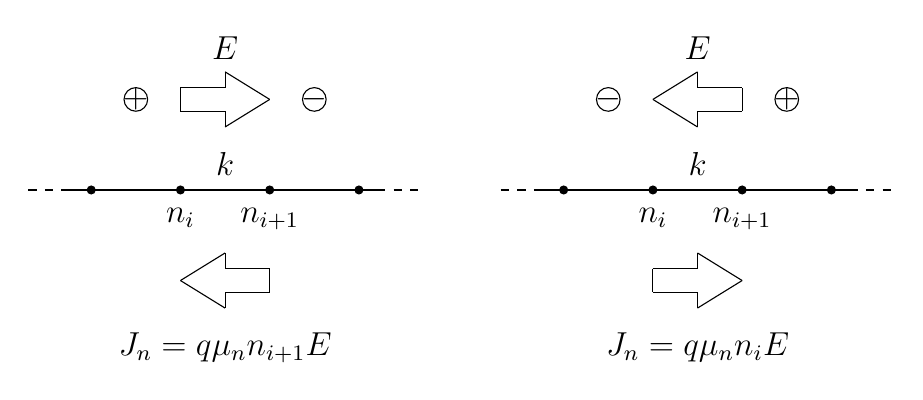
\begin{tikzpicture}
[scale=1.0]
%Solid line
\def\ax{0.5}
\def\ay{0}
\def\bx{4.5}
\def\by{0}

\def\delta{0.3}

%Dash line
\def\cx{0}
\def\cy{0}
\def\dx{5}
\def\dy{0}

\def\Np{3}
\def\step{\bx/\Np-\ax/\Np-2*\delta/\Np}
\def\halfstep{0.5*\bx/\Np-0.5*\ax/\Np-\delta/\Np}

\draw [dashed] (\cx,\cy)--(\dx,\dy);
\draw [thick](\ax,\ay)--(\bx,\by);

\draw [black,draw, fill=black] (\ax+\delta,\ay) circle [radius=0.05];
\draw [black,draw, fill=black] (\ax+\delta+\step,\ay) circle [radius=0.05];
\draw [black,draw, fill=black] (\ax+\delta+\step+\step,\ay) circle [radius=0.05];
\draw [black,draw, fill=black] (\ax+\delta+\step+\step+\step,\ay) circle [radius=0.05];

\draw [thick] (\ax+\delta +\step+\halfstep,\ay+0.05) node[above]{\large $k$};
\draw [thick] (\ax+\delta+\step,\ay-0.1) node[below]{\large $n_{i}$};
\draw [thick] (\ax+\delta+\step + \step,\ay-0.1) node[below]{\large $n_{i+1}$};


\draw [black,draw] (\ax+\delta+\halfstep,\ay+1.15) circle [radius=0.15];
\draw [black,draw] (\ax+\delta+\step + \step + \halfstep,\ay+1.15) circle [radius=0.15];
\node at (\ax+\delta + \halfstep,\ay+1.15){\large $+$};
\node at (\ax+\delta +\step + \step + \halfstep,\ay+1.15){\large $-$};

\node at (\ax+\delta +\step + \halfstep,\ay+1.8){\large $\vect{E}$};
\node at (\ax+\delta +\step + \halfstep,\ay-2.0){\large $\vect{J}_n=q\mu_n n_{i+1}\vect{E}$};

%Freccia
\draw (\ax+ \delta + \step,\ay+1)--(\ax+\delta+\step+\halfstep,\ay+1);
\draw (\ax+\delta + \step,\ay+1.3)--(\ax+\delta+\step+\halfstep,\ay+1.3);
\draw (\ax+\delta+ \step,\ay+1)--(\ax+\delta+\step,\ay+1.3);
\draw (\ax+\delta + \step +\halfstep,\ay+1.3)--(\ax+\delta+\step+\halfstep,\ay+1.5);
\draw (\ax+\delta + \step +\halfstep,\ay+1)--(\ax+\delta+\step+\halfstep,\ay+0.8);
\draw (\ax+\delta + \step +\halfstep,\ay+1.5)--(\ax+\delta+\step+\step,\ay+1.15);
\draw (\ax+\delta + \step +\halfstep,\ay+0.8)--(\ax+\delta+\step+\step,\ay+1.15);

%Freccia
\draw (\ax+ \delta + \step +\halfstep,\ay-1)--(\ax+\delta+\step +\step,\ay-1);
\draw (\ax+\delta + \step + \halfstep,\ay-1.3)--(\ax+\delta+\step + \step,\ay-1.3);
\draw (\ax+\delta+ \step + \step,\ay-1)--(\ax+\delta+\step+\step,\ay-1.3);

\draw (\ax+\delta + \step +\halfstep,\ay-1.3)--(\ax+\delta+\step+\halfstep,\ay-1.5);
\draw (\ax+\delta + \step +\halfstep,\ay-1)--(\ax+\delta+\step+\halfstep,\ay-0.8);
\draw (\ax+\delta + \step +\halfstep,\ay-1.5)--(\ax+\delta+\step,\ay-1.15);
\draw (\ax+\delta + \step +\halfstep,\ay-0.8)--(\ax+\delta+\step,\ay-1.15);


%Solid line
\def\ax{6.5}
\def\ay{0}
\def\bx{10.5}
\def\by{0}

\def\delta{0.3}

%Dash line
\def\cx{6}
\def\cy{0}
\def\dx{11}
\def\dy{0}

\def\Np{3}
\def\step{\bx/\Np-\ax/\Np-2*\delta/\Np}
\def\halfstep{0.5*\bx/\Np-0.5*\ax/\Np-\delta/\Np}

\draw [dashed] (\cx,\cy)--(\dx,\dy);
\draw [thick](\ax,\ay)--(\bx,\by);

\draw [black,draw, fill=black] (\ax+\delta,\ay) circle [radius=0.05];
\draw [black,draw, fill=black] (\ax+\delta+\step,\ay) circle [radius=0.05];
\draw [black,draw, fill=black] (\ax+\delta+\step+\step,\ay) circle [radius=0.05];
\draw [black,draw, fill=black] (\ax+\delta+\step+\step+\step,\ay) circle [radius=0.05];

\draw [thick] (\ax+\delta +\step+\halfstep,\ay+0.05) node[above]{\large $k$};
\draw [thick] (\ax+\delta+\step,\ay-0.1) node[below]{\large $n_{i}$};
\draw [thick] (\ax+\delta+\step + \step,\ay-0.1) node[below]{\large $n_{i+1}$};

\draw [black,draw] (\ax+\delta+\halfstep,\ay+1.15) circle [radius=0.15];
\draw [black,draw] (\ax+\delta+\step + \step + \halfstep,\ay+1.15) circle [radius=0.15];
\node at (\ax+\delta + \halfstep,\ay+1.15){\large $-$};
\node at (\ax+\delta +\step + \step + \halfstep,\ay+1.15){\large $+$};

\node at (\ax+\delta +\step + \halfstep,\ay+1.8){\large $\vect{E}$};
\node at (\ax+\delta +\step + \halfstep,\ay-2.0){\large $\vect{J}_n=q\mu_n n_{i}\vect{E}$};

%Freccia
\draw (\ax+ \delta + \step +\halfstep,\ay+1)--(\ax+\delta+\step +\step,\ay+1);
\draw (\ax+\delta + \step + \halfstep,\ay+1.3)--(\ax+\delta+\step + \step,\ay+1.3);
\draw (\ax+\delta+ \step + \step,\ay+1)--(\ax+\delta+\step+\step,\ay+1.3);
\draw (\ax+\delta + \step +\halfstep,\ay+1.3)--(\ax+\delta+\step+\halfstep,\ay+1.5);
\draw (\ax+\delta + \step +\halfstep,\ay+1)--(\ax+\delta+\step+\halfstep,\ay+0.8);
\draw (\ax+\delta + \step +\halfstep,\ay+1.5)--(\ax+\delta+\step,\ay+1.15);
\draw (\ax+\delta + \step +\halfstep,\ay+0.8)--(\ax+\delta+\step,\ay+1.15);

%Freccia
\draw (\ax+ \delta + \step,\ay-1)--(\ax+\delta+\step+\halfstep,\ay-1);
\draw (\ax+\delta + \step,\ay-1.3)--(\ax+\delta+\step+\halfstep,\ay-1.3);
\draw (\ax+\delta+ \step,\ay-1)--(\ax+\delta+\step,\ay-1.3);
\draw (\ax+\delta + \step +\halfstep,\ay-1.3)--(\ax+\delta+\step+\halfstep,\ay-1.5);
\draw (\ax+\delta + \step +\halfstep,\ay-1)--(\ax+\delta+\step+\halfstep,\ay-0.8);
\draw (\ax+\delta + \step +\halfstep,\ay-1.5)--(\ax+\delta+\step+\step,\ay-1.15);
\draw (\ax+\delta + \step +\halfstep,\ay-0.8)--(\ax+\delta+\step+\step,\ay-1.15);

\end{tikzpicture}


\end{center}

 \begin{equation}
\label{eq: scharfetter gummel 1D electron}
J_n^k=-q\frac{D_n}{h}
\left[ n_{i+1}\mathcal{B}\left(\frac{\Delta \varphi^k}{V_{th}}\right)- n_i\mathcal{B}\left(-\frac{\Delta \varphi^k}{V_{th}}\right)\right]  \psp{10} \forall k = 1 \, ... \, N_{elements}
\end{equation}

where $\Delta \varphi^k = \varphi_{i+1}-\varphi_i$


\subsection{Extension for the 3D case}
 
The extension of this formula for the 3D case is not trivial. We show the method for the computation of the current density of electrons (the extension for the current density of holes is quite similar).
We remark the quasi fermi formula for current density:
\begin{equation}
\label{eq: current density fermi}
\vect{J}_n=-q \mu_n n \nabla \varphi_n
\end{equation}
where $\varphi_n$ is the quasi fermi potential level. Let us write \referenzaeq{eq: current density fermi} in function of potential and in a canonic form:
\begin{equation}
\label{eq: current density canonic form}
\vect{J}_n\dfrac{ exp\left(\dfrac{\varphi_n-\varphi}{V_{th}}\right)}{q \mu_n n_i} + \nabla \varphi_n = 0
\end{equation}

Now consider a generic discretization for $\vect{J}_n$ and $\varphi_n$, for example finite element with $\mathbb{P}_1$ functions as bases (\textcolor{red}{vero che si pu´o scegliere qualsiasi discretizzazione con una qualsiasi base?}), we'll call these spaces $\left[ V_h \right]^d$ and $V_h$ (with $h$ we intend the step of discretization and $d$ is the dimension of simulation). We are able to test \referenzaeq{eq: current density canonic form} against $\vect{q}^h \in \left[ V_h \right]^d$, we choose three  different $\vect{q}^h$:

\begin{equation}
\label{eq: form of qh}
\vect{q}^h_{1,2,3} = \left\{ \begin{bmatrix} 1 \\ 0 \\ 0 \end{bmatrix}  \begin{bmatrix} 0 \\ 1 \\ 0 \end{bmatrix}  \begin{bmatrix} 0 \\ 0 \\ 1 \end{bmatrix}  \right\}
\end{equation}
We show the variational form for a generic element $K$ of the discretization:
\begin{equation}
\label{eq: variation form of current density}
\int_K \dfrac{ exp \left( \dfrac{\varphi_n-\varphi}{V_{th}} \right) }{q \mu_n n_i} \vect{J}_n^h \cdot \vect{q}^h_i \, dK
 + \int_K \nabla \varphi_n^h \cdot \vect{q}^h_i \, dK = 0 \psp{10} \forall i=1,2,3
\end{equation}

\textcolor{red}{La questione \`e: $\nabla \varphi_n^h \in \left[ V_h \right]^d$ ??. Possiamo dirlo sapendo che $\varphi_n^h \in V_h$ ??}

We know that $\nabla \varphi_n \in \mathbb{P}_0$ and without any approximation (except for the discretization) we obtain the sequent formula for the current density components:
\begin{equation}
\label{eq: first formula for J}
[\vect{J_n}]_i = - \mathbb{H}_K \left( q \mu_n n_i exp \left( \dfrac{\varphi-\varphi_n}{V_{th}} \right)  \right) \dfrac{\partial \varphi_n^h}{\partial x_i} \psp{5} i = 1...d \psp{5} \forall K \in \tau_h
\end{equation}
where $\mathbb{H}_K(f)$ is the armonic average on the elment $K$ of the function $f$.

Although resolve the armonic average with a comlete 3D integration may be expensive in calculation time and propably not necessary. One approximation of this integral would be pass from a 3D integration to 1D integration along one edge of the element $K$.
\begin{equation}
\label{eq: approzimation from 3D to edge}
\left(\dfrac{\int_K f^{-1} \, dK}{|K|} \right)^{-1} \simeq \left(\dfrac{\int_{e*} f^{-1} \, de}{|e^*|} \right)^{-1}
\end{equation}
  The approximation \referenzaeq{eq: approzimation from 3D to edge} is valid if we consider the correct edge.


Consider a quantity defined on the verteces:
\begin{equation}
\label{eq: differenza tra pot e qf}
\Phi := \varphi - 	\varphi_n
\end{equation}
which is the difference between the electrostatic potential and the quasi fermi potential level. Now for every element consider two vertices: $\vect{x}_m$ s.t. $\Phi(\vect{x}_m)=\Phi_m := min_K(\Phi)$ and $\vect{x}_M$ s.t. $\Phi(\vect{x}_M)=\Phi_M:=max_K(\Phi)$. Obviously it exists only one edge which connects these two points and on this one we perform the 1D integration \referenzaeq{eq: approzimation from 3D to edge}. First of all as we reduce the dimension is feasible to represent $\sigma(\vect{x})$ in a easier mode as follows:

\begin{equation}
\sigma_n(s) = q \mu_n n_i exp\left( \Phi_m + (\Phi_M-\Phi_m)\dfrac{s-s_m}{|e^*|} \right)
\end{equation}

where $s \in [s_m,s_M]$ is the parameter refered to the edge $e^*$ s.t. $\sigma_n(s_m)=\sigma_n(\vect{x}_m)$ and $\sigma_n(s_M)=\sigma_n(\vect{x}_M)$. We can easily resolve \referenzaeq{eq: approzimation from 3D to edge} with the substitution of variable:
\begin{equation*}
\eta := \dfrac{s-s_m}{|e^*|}
\end{equation*}

this lead us to the sequent steps of integration:

\begin{multline*}
\int_{e^*} \sigma_n^{-1} \, de = |e^*| \int_0^1 \dfrac{exp \left(-\Phi_m - (\Phi_M-\Phi_m)\eta \right)}{q\mu_n n_i} 
 \, d\eta \\
 = |e^*|\dfrac{exp (-\Phi_m)}{q\mu_n n_i} \dfrac{exp ( \Phi_m-\Phi_M)-1}{\Phi_m-\Phi_M} \\
 =  |e^*|\dfrac{exp (-\Phi_m)}{q\mu_n n_i} \dfrac{1}{\mathbf{B}(\Phi_m-\Phi_M)}
\end{multline*}

finally we obtain:
\begin{equation}
\label{eq: finally approzimation 3D to 1D}
\int_{K} \sigma_n^{-1} \, dK \simeq  q \mu_n n_i exp(\Phi_m) \mathbf{B}(\Phi_m-\Phi_M)
\end{equation}

Similar results may be obtained repeating the integration and considering $s_M$ as start point:

\begin{equation}
\int_{K} \sigma_n^{-1} \, dK \simeq  q \mu_n n_i exp(\Phi_M) \mathbf{B}(\Phi_M-\Phi_m)
\end{equation}

Numerical results (\textcolor{red}{qua sarebbe carino fare un po' di test con una parte o l'altra della formula per mettere in crisi}) shows that the best choice is e linea combination of these approzimations as follows:

\begin{equation}
\label{eq: first formula for J}
\vect{J_n}^K = -  q \mu_n  \left[ \dfrac{ n_{min} \mathbf{B}(-\Delta \Phi_{max})  + n_{max}\mathbf{B}(\Delta \Phi_{max})}{2} \right]\nabla \varphi_n^h
\end{equation}
This approach is the natrual extension of \referenzaeq{eq: scharfetter gummel 1D electron}.




\subsection{Residue Method}
\subsubsection{Contact method}
Parlare del problema del calcolo della corrente ai contatti. Infatti adoperare l'integrazione sulle superfici dei contatti risulta essere poco accurato (spiegato abbastanza bene nell'articolo Residue Method ai contatti). 

\subsubsection{Bulk method}
Now the question is: it's possible extend the residue technique at the calculation of current inside the domain? The answer at this question is not trivial. A good start point is the work of J.R. Hughes and Larson in the article "The Continuous Galerikin Method Is Locally Conservative".The aim of their work is well exposed in the title and the conclusion is that this important property (locally conservation) is ensured less than the existence of an \textbf{auxiliary flux} denoted as $H(\omega)$ (with $\omega \subseteq\Omega$). 
To extract the statement of global and local conservation from the variational formulation, thay need to be able to set the weighting function to one. Obviously this is possible if $\Gamma_g=\varnothing$. In order to include every case an extended weak formulation is presented: consider $\eta$ the set of all verteces of the discrete domain and $\eta_g$ the subset of verteces on Dirichlet boundaries.
Now we are able to define the discrete space $\mathcal{V}^h:=span\{\psi_i\}_{i\in \eta - \eta_g} $ and  $V^h:=\mathcal{V}^h \oplus span\{\psi_i\}_{i\in \eta_g}$, where $\psi_i$ is the basis function assiociated with the node $i$.
The last space is the completion of the usual finite element space ($\mathcal{V}^h$). Note that the constant function having value 1 is contained in $V^h$. The modified form of Galerkin's method is given by:

Find $u^h\in \mathcal{S}^h$ and $H^h(\Omega)\in V^h - \mathcal{V}^h$ such that

\begin{equation}
\label{eq: extended weak formulation}
(W^h,H^h(\Omega))_{\Gamma_g}=B(W^h,u^h)-L(W^h) \psp{10} \forall W^h\in V^h
\end{equation}

Note that \referenzaeq{eq: extended weak formulation} splits into two subproblems:

\begin{equation}
\label{eq: usally problem}
0=B(w^h,u^h)-L(w^h) \psp{10} \forall w^h\in \mathcal{V}^h
\end{equation}
\begin{equation}
\label{eq: problem auxiliary flux}
(W^h,H^h(\Omega))_{\Gamma_g}=B(W^h,u^h)-L(W^h) \psp{10} \forall W^h\in V^h-\mathcal{V}^h
\end{equation}

Equation \referenzaeq{eq: problem auxiliary flux} is a problem which determines $H^h(\Omega)$. In it we assume $u^h$ is already determined by \referenzaeq{eq: usally problem}.
The coefficient matrix for \referenzaeq{eq: problem auxiliary flux} is the mass matrix associated with $\Gamma_g$

\begin{equation}
\sum_{j\in \eta_g} (\psi_i,\psi_j)H^h_j(\Omega) = B(\psi_i,u^h)-L(\psi_i) \psp{10} \forall i \in \eta_g
\end{equation}

\textcolor{red}{Il prodotto sul bordo genera la medesima matrice di massa?E cosa succede nei punti che non sono di Dirichlet?Non può essere formulato in questo modo il problema?}

In ogni caso noi abbiamo provato ad estendere il secondo problema ad ogni elemento interno che intersechi o meno i bordi di Dirichlet.
Questo a cosa corrsiponde?

Abbiamo interpretato la costruzione per elemento come se in ogni elemento il problema avesse delle condizioni di dirichlet che si affacciano con gli altri elementi adiacenti.
Se assumiamo che questa procedura sia corretta allora penso che i successivi ragionamenti stiano in piedi.

Sempre nell'articolo viene testata la formulazione estesa contro la funzione test costante e si ottiene la seguente equivalenza:

\begin{equation}
\int_{\Gamma_g}H^h(\Omega) \, d\Gamma = \int_{\Gamma^+_h}(a_nu^h-h^+) \, d\Gamma - \int_{\Gamma_h^-}h^- \, d\Gamma - \int_\Omega f \, d\Omega
\end{equation}

avendo assunto ogni nodo come Dirichlet allora valgono le seguenti affermazioni:
\begin{itemize}
\item $\Gamma_g = \partial \Omega$
\item $\Gamma_h = \varnothing$
\end{itemize}

quindi possiamo affermare che per ogni elemento vale:

\begin{equation}
\int_{\partial\Omega}H^h(\Omega) \, d\Gamma =  - \int_\Omega f \, d\Omega
\end{equation}

Ora vorrei ripartire dal problema di partenza:

\begin{equation}
\begin{array}{rcl}
-\nabla \cdot \vect{J} & = & f \\
\\
\int_\Omega -\nabla \cdot \vect{J} \Psi_k \, d\Omega & = & 
\int_\Omega f \Psi_k \, d\Omega  \psp{10}  \forall k = 1 ... N_{elements}\\
\\
\int_K -\nabla \cdot \vect{J} \, d\Omega & = & \int_K f \, d\Omega  \psp{10}  \forall k = 1 ... N_{elements}\\
\\
\int_{\partial K} -\vect{J} \cdot \vect{n} \, d\Omega & = & \int_K f \, d\Omega  \psp{10}  \forall k = 1 ... N_{elements}\\

\end{array}
\end{equation}

La domanda quindi \`e possiamo in qualche modo dire che:
\begin{equation}
H^h(K) = \vect{J}\cdot \vect{n} 
\end{equation}

Entrambe le quantit\`a sono definite sul bordo dell'elemento, inoltre la ricostruzione dalle componenti normali al vettore densit\`a di corrente non \`e impossibile.
Tuttavia occorre passare prima a definire la grandezza sulle facce del tetraedro:
\begin{itemize}
\item Calcolo delle quantit\`a nodali $H^h_j(\Omega)$
\item Redistribuzione dei valori sulle facce (metodo percentuale proporzionalmente alle aree) $\bar{H}^h_j(\Omega)$
\item Ortogonalizzazione dei contributi normali alle facce $\bar{H}^h_j(\Omega) \vect{n}_j$ tramite procedura alla Grand-Shmidt $H^*_j \vect{n}_j^*$
\item Calcolo del vettore densit\`a di corrente nell'elemento $\vect{J}=\sum_{i=1}^4 H^*_j\vect{n}_j^*$
\end{itemize}


